\documentclass[11pt,letterpaper]{article}
\usepackage[utf8]{inputenc}

%----- Configuración del estilo del documento------%
\usepackage{epsfig,graphicx}
\usepackage[left=2cm,right=2cm,top=1.8cm,bottom=2.3cm]{geometry}
\usepackage{fancyhdr}
\usepackage{lastpage}
\usepackage{url}
\pagestyle{fancy}
\fancyhf{}
\rfoot{\textit{Página \thepage \hspace{1pt} de \pageref{LastPage}}}


%------ Paquetes matemáticos básicos --------%
\usepackage{amsmath}
\usepackage{amssymb}
\usepackage{amsthm}

\usepackage[spanish]{babel}
\usepackage{graphicx}
\usepackage{hyperref}

\usepackage{tabularx}
\usepackage{xcolor}
\usepackage[table]{xcolor}
\usepackage{colortbl}
\usepackage{array, multirow, multicol, tabularx}
\usepackage{tcolorbox}
\newtheorem{theorem}{Theorem}[section]
\newtheorem{corollary}{Corollary}[theorem]
\newtheorem{lemma}[theorem]{Lemma}

%------si-------%
\definecolor{B}{HTML}{FFFFFF}
\definecolor{G}{HTML}{5e5e5e}
\definecolor{R2}{HTML}{d53d40}
\definecolor{A2}{HTML}{034190}
\definecolor{V2}{HTML}{7faa50}
\newcommand{\R}{\mathbb{R}}
\newcommand{\C}{\mathcal{C}}
\newcommand{\N}{\mathbb{N}}
\newcommand{\Z}{\mathbb{Z}}
\newcommand{\Q}{\mathbb{Q}}
\renewcommand{\theenumi}{\Roman{enumi}}
\renewcommand{\labelenumi}{{\theenumi}.}

\begin{document}

%------ Encabezado -------- %

\begin{center}
    \begin{minipage}{3cm}
    	\begin{center}
    		\includegraphics[height=3.4cm]{logo_unam.png}
    	\end{center}
    \end{minipage}\hfill
    \begin{minipage}{10cm}
    	\begin{center}
    	\textbf{\large Universidad Nacional Autónoma de México}\\[0.1cm]
        \textbf{Facultad de Ciencias}\\[0.1cm]
        \textbf{\'Algebra superior 2}\\[0.1cm]
        Tarea examen 3 \\[0.1cm]
         El\'ias L\'opez Rivera\\[0.1cm]
        \texttt{ elias.lopezr\,@ciencias.unam.mx }\\[0.1cm]
        Fecha:\,\,27/07/2025
    	\end{center}
    \end{minipage}\hfill
    \begin{minipage}{3cm}
    	\begin{center}
    		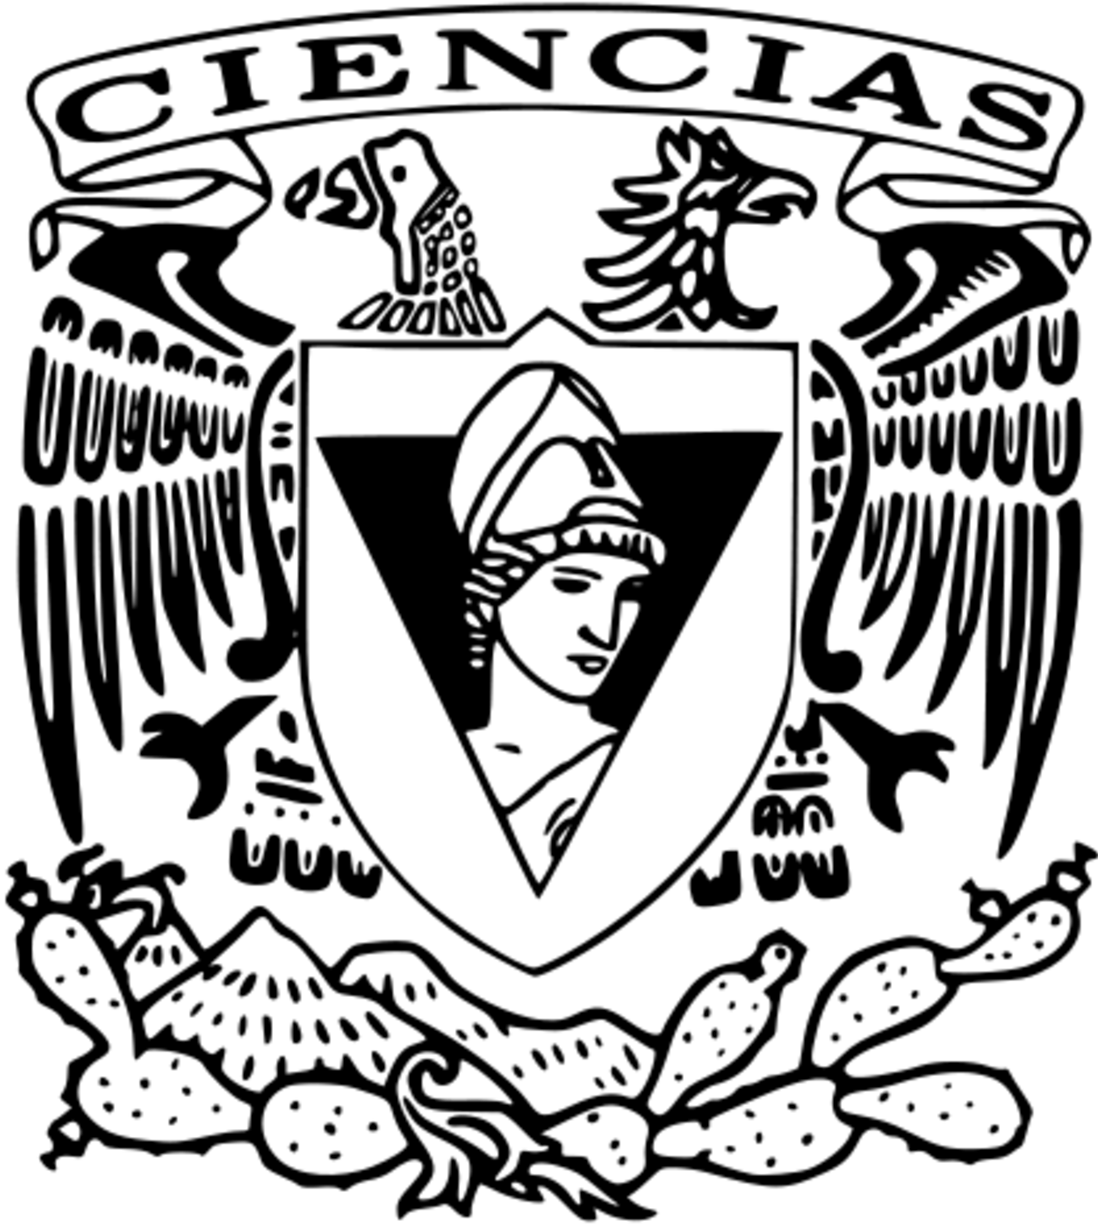
\includegraphics[height=3.4cm]{Logo_FC.png}
    	\end{center}
    \end{minipage}
\end{center}

\rule{17cm}{0.1mm}

%------ Fin de encabezado -------- %
\,\\
\section{N\'umeros reales cortaduras de Dedekind}
\begin{tcolorbox}[
	title = \textcolor{black}{\textcolor{white}{Problema 1}},]
\textit{Demuestre que la suma de los n\'umeros reales es asociativa y conmutativa
}
\end{tcolorbox}
\begin{proof}\,\\
    \,\\
\end{proof}
\begin{tcolorbox}[
	title = \textcolor{black}{\textcolor{white}{Problema 2}},]
\textit{Demuestre que si $\alpha \in \R$ y $\alpha>0$ entonces su inverso
multiplicativo $\alpha^{-1}>0$
}
\end{tcolorbox}
\begin{proof}\,\\
    \,\\
\end{proof}
\begin{tcolorbox}[
	title = \textcolor{black}{\textcolor{white}{Problema 3}},]
\textit{Sea $s\in \Q$ y $\beta$ una cortadura. Demuestre que si $s\in \beta$, entonces $\beta\in \alpha_s$
}
\end{tcolorbox}
\begin{proof}\,\\
    \,\\
\end{proof}
\section{Los n\'umeros complejos}
\begin{tcolorbox}[
	title = \textcolor{black}{\textcolor{white}{Problema 1}},]
\textit{Sean $z,w\in \C$, entonces:
\begin{enumerate}
    \item $|zw|=|z||w|$
    \item $Re(z+w)=Re(z)+Re(w)$, $Im(z+w)=Im(z)+Im(w)$
    \item $Re(-z)=-Re(z)$, $Im(-z)=-Im(z)$
\end{enumerate}
}
\end{tcolorbox}
\begin{proof}\,\\
    \,\\
\end{proof}
\begin{tcolorbox}[
	title = \textcolor{black}{\textcolor{white}{Problema 2}},]
\textit{Sean $z_1,z_2,\cdots,z_n\in \C$, $n\geq 2$ entonces:
\begin{enumerate}
    \item $\overline{z_1+z_2+\cdots+z_n}=\overline{z_1}+\overline{z_2}+\cdots+ \overline{z_n}$
    \item $\overline{(z_1)(z_2)\cdots(z_n)}=(\overline{z_1})(\overline{z_2})\cdots (\overline{z_n})$
    \item Demuestre que para toda $m\in \Z:\overline{z^m}=(\overline{z})^m$
\end{enumerate}
}
\end{tcolorbox}
\begin{proof}\,\\
    \,\\
\end{proof}
\begin{tcolorbox}[
	title = \textcolor{black}{\textcolor{white}{Problema 3}},]
\textit{Calcula las ra\'ices c\'ubicas de $8+8i$.Expresa la respuesta en
forma polar y cartesiana
}
\end{tcolorbox}
\begin{proof}\,\\
    \,\\
\end{proof}
\begin{tcolorbox}[
	title = \textcolor{black}{\textcolor{white}{Problema 4}},]
\textit{Calcula las ra\'ices c\'ubicas de $-27+27i$.Expresa la respuesta en
forma polar y cartesiana
}
\end{tcolorbox}
\begin{proof}\,\\
    \,\\
\end{proof}

\begin{tcolorbox}[
	title = \textcolor{black}{\textcolor{white}{Problema 5}},]
\textit{Calcula las ra\'ices cuartas de $32+32i$
}
\end{tcolorbox}
\begin{proof}\,\\
    \,\\
\end{proof}
\begin{tcolorbox}[
	title = \textcolor{black}{\textcolor{white}{Problema 6}},]
\textit{Calcula las ra\'ices quintas de $-1+i$.Escribe los resultados en terminos de su argumento
y su modulo
}
\end{tcolorbox}
\begin{proof}\,\\
    \,\\
\end{proof}
\begin{tcolorbox}[
	title = \textcolor{black}{\textcolor{white}{Problema 7}},]
\textit{Calcula las ra\'ices sextas de $64$
}
\end{tcolorbox}
\begin{proof}\,\\
    \,\\
\end{proof}
\begin{tcolorbox}[
	title = \textcolor{black}{\textcolor{white}{Problema 8}},]
\textit{Describa geometricamente los siguientes conjuntos :
\begin{enumerate}
    \item $\{z\in C|\,Im(z)>0\}$
    \item $\{z\in C|\,z=-\overline{z}\}$
    \item $\{z\in C|\,z^{-1}=\overline{z}\}$
\end{enumerate}
}
\end{tcolorbox}
\end{document}